% Pour compiler :
%$ lualatex $basename

\documentclass[12pt, tikz]{standalone}

\begin{document}
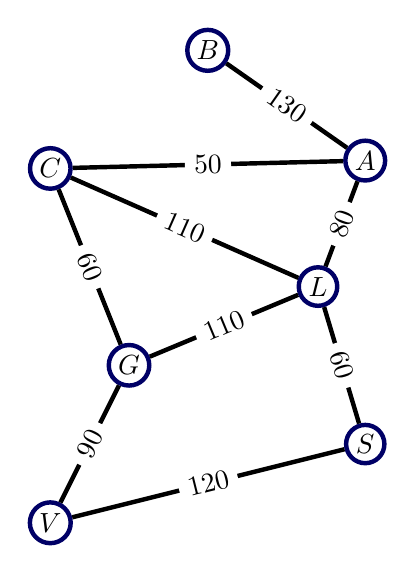
\begin{tikzpicture}[scale=1.0, ultra thick]
\tikzstyle{sommet} = [circle, draw=black!60!blue, inner sep=1.5pt]
\tikzstyle{etiquette} = [midway, fill=white, sloped, anchor=center]
\node[sommet] (A) at (4, 3.6) {$A$};
\node[sommet] (B) at (2,5) {$B$};
\node[sommet] (C) at (0,3.5) {$C$};
\node[sommet] (L) at (3.4,2) {$L$};
\node[sommet] (G) at (1,1) {$G$};
\node[sommet] (V) at (0,-1) {$V$};
\node[sommet] (S) at (4,0) {$S$};
\draw (A) -- (B) node[etiquette]{130};
\draw (A) -- (C) node[etiquette]{50};
\draw (A) -- (L) node[etiquette]{80};
\draw (C) -- (G) node[etiquette]{60};
\draw (C) -- (L) node[etiquette]{110};
\draw (G) -- (L) node[etiquette]{110};
\draw (G) -- (V) node[etiquette]{90};
\draw (L) -- (S) node[etiquette]{60};
\draw (S) -- (V) node[etiquette]{120};
\end{tikzpicture}

\end{document}
